\section{TCP Client - Server}
\subsection{Aim}
To implement Client-Server communication using Socket Programming and TCP as
transport layer protocol.

\subsection{Theory}
\textbf{TCP (Transmission Control Protocol)} is one of the main protocols in TCP/IP
networks. Transmission control protocol (TCP) is a network communication protocol designed to send data packets over the Internet. TCP is a transport layer protocol
in the OSI layer and is used to create a connection between remote computers by
transporting and ensuring the delivery of messages over supporting networks and
the Internet.\\
It is a connection-oriented protocol, which means that a connection is established
and maintained until the application programs at each end have finished exchanging
messages.\\
TCP programs are implemented in two parts:\\
• \textbf{Server} : A server program listens for a connection. On getting a request,
the server accepts a connection. After the connection is established, server
and client can exchange messages.\\
• \textbf{Client} : A client program requests some service. A client program request
for some resources to the server and server responds to that request. Client
initiates the connection establishment. The server accepts connection and
client can request services by exchanging messages.\\
\textbf{Sockets}
Implementation of the above two programs (Client and Server) is to be done with
the help of sockets. A socket is one endpoint of a two-way communication link
between two programs running on the network. Client program and server program
create and use sockets to communicate with each other.

\subsection{Algorithm}
\subsubsection{Server}
\begin{verbatim}
1 START
2 Configure socket details
3 Bind the address struct to the socket using bind()
4 Listen to the socket
5 A new socket for the incoming connection is created using accept()
6 Send message to the incoming connection using send()
7 STOP
\end{verbatim}

\subsubsection{Client}
\begin{verbatim}
1 START
2 Create the socket using socket()
3 Configure the socket details
4 Connect the socket to server using connect()
5 Recieve the message from server using recv()
6 Print the recieved message
7 STOP
\end{verbatim}

\subsection{Source Code}
\subsubsection{Server}
\begin{lstlisting}[language=C]
#include <stdio.h>
#include <stdlib.h>
#include <sys/types.h>
#include <sys/socket.h>
#include <netinet/in.h>
#include <errno.h>
#include <unistd.h>
#include <string.h>

// The number of connection requests to be queued, all exceeding
// connections will be rejected
#define QUEUE_LENGTH 5 

// sockaddr acts as a general structure, while sockaddr_in is specific
// for internet sockets
typedef struct sockaddr sockaddr_t; 
typedef struct sockaddr_in sockaddr_in_t;

extern int errno;

const int PORT = 8080;
const char *MESSAGE = "Hello world";

// Create a socket with TCP as protocol
void create_socket(int *socket_fd) {
  if((*socket_fd = socket(AF_INET, SOCK_STREAM, 0)) == -1) {
    perror("Failed to create socket");
    fprintf(stderr, "Errno: %d\n", errno);
    exit(EXIT_FAILURE);
  }

  printf("Socket created with TCP protocol\n");
}

// Configure the socket
void configure_socket(const int *socket_fd) {
  sockaddr_in_t server_addr;

  // For sockaddr_in, sin_family is always AF_INET (for TCP and UDP)
  server_addr.sin_family = AF_INET;
  
  // Accept any incoming message irrespective of IP
  server_addr.sin_addr.s_addr = htonl(INADDR_ANY); 

  // Listen to port specified by PORT
  server_addr.sin_port = htons(PORT);

  if(bind(*socket_fd, (sockaddr_t *)&server_addr, sizeof(server_addr)) == -1) {
    perror("Failed to bind socket configuration");
    fprintf(stderr, "Errno: %d\n", errno);
    exit(EXIT_FAILURE);
  }

  printf("Socket binding successful\n");
}

// Listen and accept connection from clients
void connect_client(const int *socket_fd, int *client_socket_fd) {
  sockaddr_in_t client; // For storing client details

  // Listen for connection from client
  if(listen(*socket_fd, QUEUE_LENGTH) == -1) {
    perror("Listening failed");
    fprintf(stderr, "Errno: %d\n", errno);
    exit(EXIT_FAILURE);
  }

  printf("Server listening\n");
  
  socklen_t len = sizeof(client);
  // Accept connection from client
  if((*client_socket_fd = 
              accept(*socket_fd, (sockaddr_t *)&client, &len)) == -1) {
    perror("Accepting connection failed");
    fprintf(stderr, "Errno: %d\n", errno);
    exit(EXIT_FAILURE);
  }

  printf("Server accepted client\n");
}

// Send the MESSAGE to client
void send_message(const int *client_socket_fd) {
  ssize_t message_send_total = 0, message_send;

  while(message_send_total < sizeof(MESSAGE)) {
    message_send = send(
      *client_socket_fd, 
      MESSAGE+message_send_total, 
      strlen(MESSAGE+message_send_total)+1, 
      0
    );

    if(message_send == -1) {
      perror("Sending message failed");
      fprintf(stderr, "Errno: %d\n", errno);
      exit(EXIT_FAILURE);
    }
    message_send_total += message_send;
  }

  printf("Sending message success. Send %d bytes\n", message_send_total);
}

// Close the socket
void close_socket(int *socket_fd) {
  close(*socket_fd);
  printf("Socket closed\n");
}

int main() {
  int socket_fd; // The file descriptor for socket
  int client_socket_fd; // The file descriptor for client

  create_socket(&socket_fd);
  configure_socket(&socket_fd);
  connect_client(&socket_fd, &client_socket_fd);
  send_message(&client_socket_fd);
  close_socket(&socket_fd);
  
  return 0;
}
\end{lstlisting}

\subsubsection{Client}
\begin{lstlisting}[language=C]
#include <stdio.h>
#include <stdlib.h>
#include <sys/types.h>
#include <sys/socket.h>
#include <netinet/in.h>
#include <arpa/inet.h>
#include <errno.h>
#include <netdb.h>

#define MESSAGE_LENGTH 255

  // The number of connection requests to be queued, all exceeding
  // connections will be rejected
  typedef struct sockaddr sockaddr_t;
  typedef struct sockaddr_in sockaddr_in_t;
  
  extern int errno;
  
  const int PORT = 8080;
  
  // Create a TCP socket
  void create_socket(int *socket_fd) {
    if((*socket_fd = socket(AF_INET, SOCK_STREAM, 0)) == -1) {
      perror("Failed to create socket");
      fprintf(stderr, "Errno: %d\n", errno);
      exit(EXIT_FAILURE);
    }
  
    printf("Socket created successfully\n");
  }
  
  // Connect the socket to server
  void connect_server(int *socket_fd) {
    sockaddr_in_t client_addr;
  
    client_addr.sin_port = htons(PORT);
    client_addr.sin_addr.s_addr = inet_addr("127.0.0.1");
    client_addr.sin_family = AF_INET;
  
    if(connect(
      *socket_fd, (sockaddr_t *)&client_addr, sizeof(client_addr)
    ) == -1) {
      perror("Failed to connect to socket");
      fprintf(stderr, "Errno: %d\n", errno);
      exit(EXIT_FAILURE);
    }
  
    printf("Connected to socket\n");
  }
  
  // Read message from server
  void read_message(int *socket_fd) {
    char message[MESSAGE_LENGTH];
    ssize_t message_recieved, message_recieved_total = 0;
    
    while(message_recieved && message[message_recieved_total] != '\0') {
      message_recieved = recv(
        *socket_fd, 
        (message+message_recieved_total), 
        MESSAGE_LENGTH, 
        0
      );
  
      if(message_recieved == -1) {
        perror("Recieving message failed");
        fprintf(stderr, "Errno: %d\n", errno);
        exit(EXIT_FAILURE);
      }
  
      message_recieved_total += message_recieved;
      printf("%d", message_recieved);
    }
    
    printf(
      "Recieving message success. Recieved %d bytes\n", 
      message_recieved_total
    );
    printf("Recieved message: %s\n", message);
  }
  
  int main() {
    int socket_fd;
  
    create_socket(&socket_fd);
    connect_server(&socket_fd);
    read_message(&socket_fd);
  
    return 0;
  }  
\end{lstlisting}

\begin{center}
	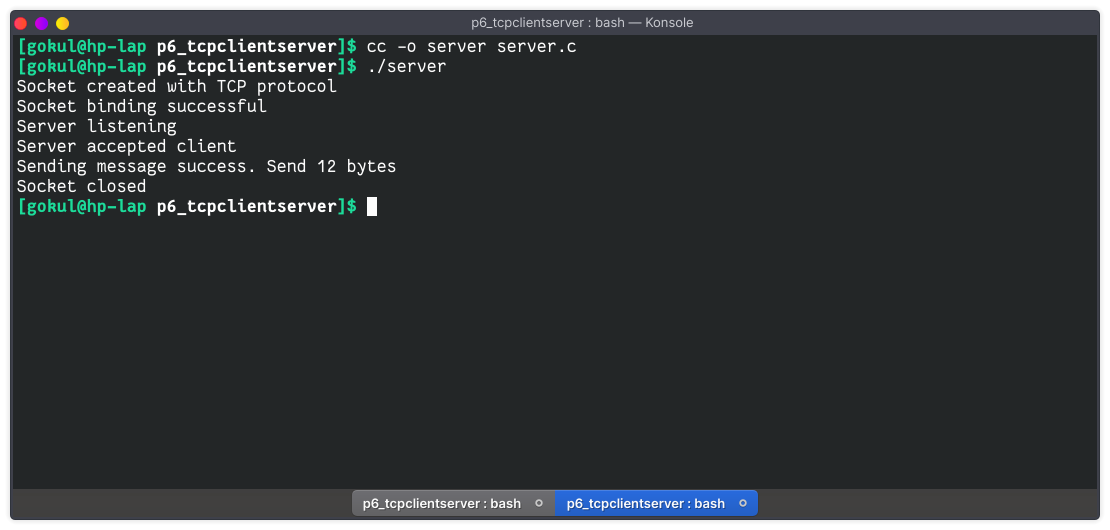
\includegraphics[width=0.90\textwidth]{img/p7/ss1.png}
	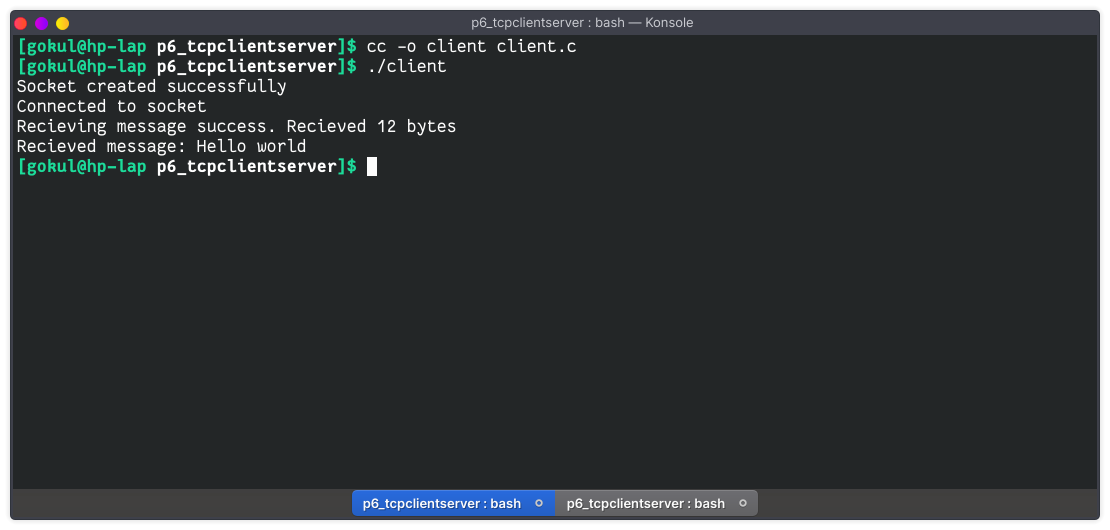
\includegraphics[width=0.90\textwidth]{img/p7/ss2.png}
\end{center}


\subsection{Result}
The above programs were executed and its output were verified